\begin{name}
	{\tenchude}
	{ĐỀ KSCL SỞ NINH BÌNH}
	{LỚP TOÁN THẦY PHÁT}
	{\lq\lq  The beautiful thing about learning is that no one can take it away from you.\rq\rq}
\end{name}

\Opensolutionfile{ansbook}[ans/ansb\currfilebase]
\caulc
\Opensolutionfile{ans}[ans/ans\currfilebase-Phan-I]
\begin{ex}%[2H2N2-2]%[DỰ ÁN TEX ĐỀ THI THỬ THPT 2026]%[NHẬT THIỆN]
	Trong không gian với hệ trục tọa độ $Oxyz$, cho hai điểm $A(1;3;5)$ và $B(5;-3;1)$. Trung điểm của đoạn thẳng $AB$ có tọa độ là
	\choice
	{\True $(3;0;3)$}
	{$(6;0;6)$}
	{$(-2;3;2)$}
	{$(-4;6;4)$}
	\loigiai{
		Ta có $\heva{&x_I=\dfrac{x_A+x_B}{2}\\&y_I=\dfrac{y_A+y_B}{2}\\&z_I=\dfrac{z_A+z_B}{2}}\Rightarrow I(3;0;3)$.
	}
\end{ex}

\begin{ex}%[2D1N1-2]%[DỰ ÁN TEX ĐỀ THI THỬ THPT 2026]%[NHẬT THIỆN]
	Cho hàm số $y=f(x)$ liên tục trên $\mathbb{R}$, có bảng xét dấu đạo hàm như sau:
	\begin{center}
		
\begin{tikzpicture}[scale=1, font=\footnotesize, line join=round, line cap=round, >=stealth]
			\tkzTabInit[lgt=1,espcl=2]
			{$x$ /0.6, $f'(x)$ /0.6}
			{$-\infty$ , $-2$,$0$,$2$, $+\infty$}
			\tkzTabLine{,+,0,-,d,-,0,+,}
		\end{tikzpicture}
	\end{center}
	Khẳng định nào dưới đây đúng?
	\choice
	{Hàm số nghịch biến trên khoảng $(-\infty;0)$}
	{Hàm số đồng biến trên khoảng $(1;+\infty)$}
	{\True Hàm số đồng biến trên khoảng $(-\infty;-2)$}
	{Hàm số nghịch biến trên khoảng $(0;4)$}
	\loigiai{
		Từ bảng biến thiên, ta thấy $f'(x)>0$ với $x\in(-\infty;-2)$ nên hàm số đồng biến trên khoảng $(-\infty;-2)$.
	}
\end{ex}

\begin{ex}%[2H2N2-4]%[DỰ ÁN TEX ĐỀ THI THỬ THPT 2026]%[NHẬT THIỆN]
	Trong không gian với hệ trục tọa độ $Oxyz$, cho hai vectơ $\overrightarrow{u}=(2;-1;-2)$ và $\overrightarrow{v}=(1;1;3)$. Giá trị của $\overrightarrow{u}\cdot \overrightarrow{v}$ bằng
	\choice
	{$9$}
	{$7$}
	{$3\sqrt{11}$}
	{\True $-5$}
	\loigiai{
		Ta có $\overrightarrow{u}\cdot \overrightarrow{v}=2\cdot 1+(-1)\cdot 1+(-2)\cdot 3=-5$.
	}
\end{ex}

\begin{ex}%[2D1H3-1]%[DỰ ÁN TEX ĐỀ THI THỬ THPT 2026]%[NHẬT THIỆN]
	Giá trị lớn nhất của hàm số $y=x^3-3x+2$ trên đoạn $[0;3]$ bằng
	\choice
	{$2$}
	{$3$}
	{\True $20$}
	{$0$}
	\loigiai{
		Ta có $y'=3x^2-3$.\\
		$y'=0\Leftrightarrow3x^2-3=0\Leftrightarrow \hoac{&x=1 \quad \text{ (thỏa mãn)}\\ &x=-1 \quad \text{ (loại)}}$ với $x\in[0;3]$.\\
		Xét $y(1)=0$; $y(0)=2$; $y(3)=20$.\\
		Vậy $\max\limits_{[0;3]}y=20$.
	}
\end{ex}

\begin{ex}%[2H2N2-2]%[DỰ ÁN TEX ĐỀ THI THỬ THPT 2026]%[NHẬT THIỆN]
	Trong không gian với hệ trục tọa độ $Oxyz$, hình chiếu vuông góc của điểm $M(2;-1;3)$ trên trục $Oy$ là điểm có tọa độ
	\choice
	{$(0;0;3)$}
	{\True $(0;-1;0)$}
	{$(2;0;0)$}
	{$(2;0;3)$}
	\loigiai{
		Hình chiếu của $M$ trên trục $Oy$ là $M'(0;-1;0)$.
	}
\end{ex}

\begin{ex}%[2D3N1-1]%[DỰ ÁN TEX ĐỀ THI THỬ THPT 2026]%[NHẬT THIỆN]
	Cho mẫu số liệu ghép nhóm có tứ phân vị là $Q_1$, $Q_2$, $Q_3$. Khoảng tứ phân vị $\Delta_{Q}$ của mẫu số liệu xác định bởi công thức nào sau đây?
	\choice
	{\True $\Delta_{Q}=Q_3-Q_1$}
	{$\Delta_{Q}=Q_3-Q_2$}
	{$\Delta_{Q}=Q_2-Q_1$}
	{$\Delta_{Q}=Q_1-Q_3$}
	\loigiai{
		Khoảng tứ phân vị $\Delta_{Q}=Q_3-Q_1$.
	}
\end{ex}

\begin{ex}%[2D1N4-1]%[DỰ ÁN TEX ĐỀ THI THỬ THPT 2026]%[NHẬT THIỆN]
	Cho hàm số $f(x)$ có bảng biến thiên như hình vẽ sau
	\begin{center}
		
\begin{tikzpicture}[scale=1, font=\footnotesize, line join=round, line cap=round, >=stealth]
			\tkzTabInit[lgt=1,espcl=2]
			{$x$ /0.6, $f'(x)$ /0.6,$f(x)$ /2}
			{$-\infty$ , $-1$,$1$,$3$, $+\infty$}
			\tkzTabLine{,-,d,+,d,-,0,+,}
			\tkzTabVar{+/$+\infty$ ,-D-/$-\infty$/$-2$, +D+/$4$/$1$,-/$-5$,+/$0$}
		\end{tikzpicture}
	\end{center}
	Tổng số đường tiệm cận đứng và tiệm cận ngang của đồ thị hàm số $y=f(x)$ là
	\choice
	{$3$}
	{$1$}
	{$4$}
	{\True $2$}
	\loigiai{
		Dựa vào bảng biến thiên ta thấy đồ thị hàm số có một tiệm cận ngang là $y=0$ và một tiệm cận đứng $x=-1$.\\
		Suy ra đồ thị hàm số có $2$ đường tiệm cận.
	}
\end{ex}

\begin{ex}%[2D1N2-2]%[DỰ ÁN TEX ĐỀ THI THỬ THPT 2026]%[NHẬT THIỆN]
	\immini{Cho hàm số bậc ba $y=f(x)$ có đồ thị như hình vẽ bên.
	Giá trị cực đại của hàm số đã cho là
	\choice
	{$1$}
	{$-1$}
	{\True $2$}
	{$-2$}}{
	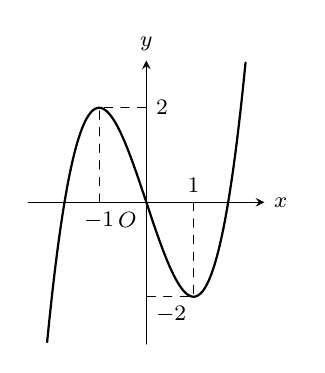
\begin{tikzpicture}[scale=0.6, font=\footnotesize, line join=round, line cap=round, >=stealth]
		\draw[->] (-2.5,0) -- (2.5,0) node[right] {$x$};
		\draw[->] (0,-3) -- (0,3) node[above] {$y$};
		\node[below left] at (0,0) {$O$};
		\draw[thick, domain=-2.1:2.1, samples=100, smooth] plot (\x, {(\x)^3 - 3*\x});
		\draw[dashed] (-1,0) node[below] {$-1$} -- (-1,2) -- (0,2) node[right] {$2$};
		\draw[dashed] (1,0) node[above] {$1$} -- (1,-2) -- (0,-2) node[below right] {$-2$};
	\end{tikzpicture}
	}
	\loigiai{
		Từ đồ thị hàm số suy ra giá trị cực đại của hàm số đã cho là $y_{\text{CĐ}}=2$.
	}
\end{ex}

\begin{ex}%[2D1H4-1]%[DỰ ÁN TEX ĐỀ THI THỬ THPT 2026]%[NHẬT THIỆN]
	Phương trình đường tiệm cận xiên của đồ thị hàm số $y=\dfrac{x^2+x-3}{x+1}$ là
	\choice
	{$y=x+1$}
	{\True $y=x$}
	{$y=x-3$}
	{$y=2x$}
	\loigiai{
		Ta có $y=\dfrac{x^2+x-3}{x+1}=x-\dfrac{3}{x+1}$.\\
		Suy ra $\lim\limits_{x\rightarrow+\infty}(y-x)=\lim\limits_{x\rightarrow+\infty}\dfrac{-3}{x+1}=0$; $\lim\limits_{x\rightarrow-\infty}(y-x)=\lim\limits_{x\rightarrow-\infty}\dfrac{-3}{x+1}=0$.\\
		Vậy tiệm cận xiên của đồ thị hàm số là đường thẳng $y=x$.
	}
\end{ex}

\begin{ex}%[2D3H1-2]%[DỰ ÁN TEX ĐỀ THI THỬ THPT 2026]%[NHẬT THIỆN]
	Điểm kiểm tra môn Toán của học sinh lớp 12A được ghi lại ở bảng số liệu ghép nhóm sau:
	\begin{center}
		\begin{tabular}{|c|c|c|c|c|c|}
			\hline
			Nhóm & $[0;2)$ & $[2;4)$ & $[4;6)$ & $[6;8)$ & $[8;10]$ \\
			\hline
			Tần số & $2$ & $11$ & $14$ & $9$ & $3$ \\
			\hline
		\end{tabular}
	\end{center}
	Khoảng biến thiên của mẫu số liệu ghép nhóm trên là
	\choice
	{\True $10$}
	{$8$}
	{$12$}
	{$14$}
	\loigiai{
		Khoảng biến thiên $R=10-0=10$.
	}
\end{ex}

\begin{ex}%[2H2H2-4]%[DỰ ÁN TEX ĐỀ THI THỬ THPT 2026]%[NHẬT THIỆN]
	Trong không gian với hệ tọa độ $Oxyz$, cho hai vectơ $\overrightarrow{u}=(2;3;-1)$ và $\overrightarrow{v}=(1;3;2)$. Độ dài của vectơ $\overrightarrow{w}=2\overrightarrow{u}-3\overrightarrow{v}$ là
	\choice
	{$\sqrt{290}$}
	{$290$}
	{$74$}
	{\True $\sqrt{74}$}
	\loigiai{
		Ta có: $2\overrightarrow{u}=(4;6;-2)$; $3\overrightarrow{v}=(3;9;6)\Rightarrow\overrightarrow{w}=2\overrightarrow{u}-3\overrightarrow{v}=(1;-3;-8)$.\\
		Vậy $|\overrightarrow{w}|=\sqrt{1+(-3)^2+(-8)^2}=\sqrt{74}$.
	}
\end{ex}

\begin{ex}%[2D1H5-7]%[DỰ ÁN TEX ĐỀ THI THỬ THPT 2026]%[NHẬT THIỆN]
	Đồ thị hàm số $y=\dfrac{2x+3}{x-1}$ có tâm đối xứng là điểm
	\choice
	{$N(3;-1)$}
	{\True $P(1;2)$}
	{$Q\left(1;-\dfrac{3}{2}\right)$}
	{$M(2;-1)$}
	\loigiai{
		Đồ thị hàm số đã cho có tiệm cận đứng $x=1$ và tiệm cận ngang $y=2$ nên giao điểm hai tiệm cận là $P(1;2)$ là tâm đối xứng.
	}
\end{ex}

\Closesolutionfile{ans}
\cauds
\Opensolutionfile{ans}[ans/ans\currfilebase-Phan-II]

\begin{ex}%[2D1H5-5]%[DỰ ÁN TEX ĐỀ THI THỬ THPT 2026]%[NHẬT THIỆN]
	\immini{Cho hàm số bậc bốn $y=f(x)$. Hàm số $y=f'(x)$ có đồ thị như hình vẽ bên.
	\choiceTF
	{\True Hàm số $y=f(x)$ nghịch biến trên khoảng $(-\infty;-2)$}
	{\True Hàm số $y=f(x)$ có ba điểm cực trị}
	{Giá trị nhỏ nhất của hàm số trên đoạn $[-2;2]$ là $f(0)$}
	{Biết $f(0)>0$. Khi đó phương trình $f(x)=0$ có tối đa ba nghiệm phân biệt}}{
	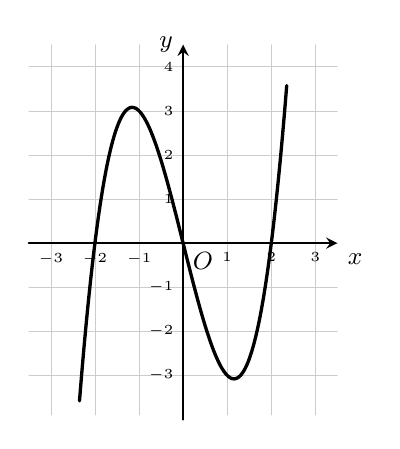
\begin{tikzpicture}[scale=0.7, font=\footnotesize, line join=round, line cap=round, >=stealth]
		\begin{scope}[scale=.8]
			\draw[help lines, step=1, gray!40] (-3.5,-3.9) grid (3.5,4.5);
			\draw[->, thick] (-3.5,0) -- (3.5,0) node[below right] {\small $x$};
			\draw[->, thick] (0,-4) -- (0,4.5) node[left] {\small $y$};
			\node[below right] at (0,0) {\small $O$};
			\foreach \x in {-3,-2,-1,1,2,3}
			\node[below, font=\tiny] at (\x,0) {$\x$};
			\foreach \y in {-3,-2,-1,1,2,3,4}
			\node[left, font=\tiny] at (0,\y) {$\y$};
			\draw[very thick, smooth, domain=-2.35:2.35, samples=100] 
			plot (\x, {(\x)^3 - 4*\x});
		\end{scope}
	\end{tikzpicture}
	}
	\loigiai{
		Từ đồ thị hàm số $f'(x)$, ta có bảng biến thiên của hàm số $y=f(x)$
		\begin{center}
			
\begin{tikzpicture}[scale=1, font=\footnotesize, line join=round, line cap=round, >=stealth]
				\tkzTabInit[lgt=1,espcl=2]
				{$x$ /0.6, $y'$ /0.6,$y$ /2}
				{$-\infty$ , $-2$,$0$,$2$, $+\infty$}
				\tkzTabLine{,-,0,+,0,-,0,+,}
				\tkzTabVar{+/$+\infty$ ,-/,+/,-/,+/$+\infty$}
			\end{tikzpicture}
		\end{center}
		\begin{itemchoice}
			\itemch Hàm số nghịch biến trên khoảng $(-\infty;-2)$.
			\itemch Dựa vào bảng biến thiên, hàm số $y=f(x)$ có ba điểm cực trị.
			\itemch Trên đoạn $[-2;2]$, hàm số $y=f(x)$ có giá trị lớn nhất bằng $f(0)$.
			\itemch Vì $f(0)>0$, dựa vào BBT phương trình $f(x)=0$ có hai nghiệm phân biệt.
		\end{itemchoice}
	}
\end{ex}

\begin{ex}%[2D1H2-1]%[DỰ ÁN TEX ĐỀ THI THỬ THPT 2026]%[NHẬT THIỆN]
	Cho hàm số $y=\dfrac{x^2+x+1}{x+1}$
	\choiceTF
	{Hàm số $y=f(x)$ đồng biến trên $\mathbb{R}$}
	{$y'=\dfrac{x^2-2x}{(x+1)^2}$, $\forall x\ne-1$}
	{\True Hàm số có bảng biến thiên như sau
	\begin{center}
		
\begin{tikzpicture}[scale=1, font=\footnotesize, line join=round, line cap=round, >=stealth]
			\tkzTabInit[lgt=1,espcl=2]
			{$x$ /0.6, $f'(x)$ /0.6,$f(x)$ /2}
			{$-\infty$ , $-2$,$-1$,$0$, $+\infty$}
			\tkzTabLine{,+,0,-,d,-,0,+,}
			\tkzTabVar{-/$-\infty$ ,+/$-3$,-D+/$-\infty$/$+\infty$,-/$1$,+/$+\infty$}
		\end{tikzpicture}
	\end{center}
	}
	{\True Khoảng cách giữa hai điểm cực trị của đồ thị hàm số bằng $2\sqrt{5}$}
	\loigiai{
		Điều kiện xác định $x+1\ne0\Leftrightarrow x\ne-1$.\\
		Ta có $y=x+\dfrac{1}{x+1}$.\\
		Suy ra $y'=\dfrac{x^2+2x}{(x+1)^2}$, $\forall x\ne-1$.\\
		Xét $y'=0\Leftrightarrow x^2+2x=0\Leftrightarrow \hoac{&x=0\\ &x=-2.}$\\
		Bảng biến thiên
		\begin{center}
			
\begin{tikzpicture}[scale=1, font=\footnotesize, line join=round, line cap=round, >=stealth]
				\tkzTabInit[lgt=1,espcl=2]
				{$x$ /0.6, $f'(x)$ /0.6,$f(x)$ /2}
				{$-\infty$ , $-2$,$-1$,$0$, $+\infty$}
				\tkzTabLine{,+,0,-,d,-,0,+,}
				\tkzTabVar{-/$-\infty$ ,+/$-3$,-D+/$-\infty$/$+\infty$,-/$1$,+/$+\infty$}
			\end{tikzpicture}
		\end{center}
		\begin{itemchoice}
			\itemch 
			Hàm số đồng biến trên $(-\infty;-2)$ và $(0;+\infty)$.
			\itemch Ta có $y'=\dfrac{x^2+2x}{(x+1)^2}$, $\forall x\ne-1$.\\
			\itemch 	Bảng biến thiên
			\begin{center}
				
\begin{tikzpicture}[scale=1, font=\footnotesize, line join=round, line cap=round, >=stealth]
					\tkzTabInit[lgt=1,espcl=2]
					{$x$ /0.6, $f'(x)$ /0.6,$f(x)$ /2}
					{$-\infty$ , $-2$,$-1$,$0$, $+\infty$}
					\tkzTabLine{,+,0,-,d,-,0,+,}
					\tkzTabVar{-/$-\infty$ ,+/$-3$,-D+/$-\infty$/$+\infty$,-/$1$,+/$+\infty$}
				\end{tikzpicture}
			\end{center}
			\itemch Hàm số có hai điểm cực trị $A(-2;-3)$, $B(0;1)$.\\
			Suy ra $AB=\sqrt{2^2+4^2}=2\sqrt{5}$.
		\end{itemchoice}
	}
\end{ex}

\begin{ex}%[2H2H2-4]%[DỰ ÁN TEX ĐỀ THI THỬ THPT 2026]%[NHẬT THIỆN]
	Trong không gian với hệ tọa độ $Oxyz$, cho tam giác $ABC$ với $A(3;0;0)$, $B(0;6;0)$, $C(0;0;-9)$.
	\choiceTF
	{\True Tọa độ trọng tâm $G$ của tam giác $ABC$ là $(1;2;-3)$}
	{ $\overrightarrow{GA}=(-2;2;-3)$}
	{\True $GA=\sqrt{17}$}
	{$\cos \widehat{AGB}=\dfrac{1}{\sqrt{442}}$}
	\loigiai{
		\begin{itemchoice}
			\itemch Ta có $\heva{&x_{G}=\dfrac{3+0+0}{3}=1\\& y_{G}=\dfrac{0+6+0}{3}=2\\& z_{G}=\dfrac{0+0-9}{3}=-3} \Rightarrow G(1;2;-3)$.
			\itemch $\overrightarrow{GA}=(3-1; 0-2; 0-(-3)) = (2;-2;3)$.
			\itemch $GA=\sqrt{2^2+(-2)^2+3^2}=\sqrt{17}$.
			\itemch Ta có $\overrightarrow{GA}=(2;-2;3)$ và $\overrightarrow{GB}=(-1;4;3)$.\\
			Suy ra $\cos \widehat{AGB}=\dfrac{\overrightarrow{GA}\cdot \overrightarrow{GB}}{\left|\overrightarrow{GA}\right|\cdot \left|\overrightarrow{GB}\right|}=\dfrac{2\cdot (-1)+(-2)\cdot 4+3\cdot 3}{\sqrt{17}\cdot \sqrt{(-1)^2+4^2+3^2}}=-\dfrac{1}{\sqrt{442}}$.
		\end{itemchoice}
	}
\end{ex}

\begin{ex}%[2D3H2-3]%[DỰ ÁN TEX ĐỀ THI THỬ THPT 2026]%[NHẬT THIỆN]
	Thống kê thời gian trung bình sử dụng máy vi tính trong một ngày của nhân viên công ty X cho bởi bảng số liệu ghép nhóm sau:
	\begin{center}
		\begin{tabular}{|c|c|c|c|c|c|}
			\hline
			Thời gian (phút) & $[30;60)$ & $[60;90)$ & $[90;120)$ & $[120;150)$ & $[150;180)$ \\
			\hline
			Số nhân viên & $3$ & $5$ & $5$ & $25$ & $2$ \\
			\hline
		\end{tabular}
	\end{center}
	\choiceTF
	{\True Số phần tử (cỡ mẫu) của mẫu số liệu trên là $n=40$}
	{\True Số trung bình cộng của mẫu số liệu trên bằng $118{,}5$}
	{Phương sai của mẫu số liệu trên bằng $945$}
	{Độ lệch chuẩn của mẫu số liệu trên bằng $3\sqrt{105}$}
	\loigiai{
		\begin{itemchoice}
			\itemch $n=3+5+5+25+2=40$.
			\itemch 
			\begin{center}
				\begin{tabular}{|c|c|c|c|c|c|}
					\hline
					Thời gian (phút) & $[30;60)$ & $[60;90)$ & $[90;120)$ & $[120;150)$ & $[150;180)$ \\
					\hline
					Giá trị đại diện& $45$& $75$& $105$& $135$& $165$.\\
					\hline
					Số nhân viên & $3$ & $5$ & $5$ & $25$ & $2$ \\
					\hline
				\end{tabular}
			\end{center}
			
			$\overline{x}=\dfrac{45\cdot 3+75\cdot 5+105\cdot 5+135\cdot 25+165\cdot 2}{40}=118{,}5$.
			\itemch Phương sai $S^2=\dfrac{1}{40}(3\cdot45^2+5\cdot75^2+5\cdot105^2+25\cdot135^2+2\cdot165^2) - 118{,}5^2 = 942{,}75$.
			\itemch $S=\sqrt{942{,}75}=\dfrac{3\sqrt{419}}{2}$.
		\end{itemchoice}
	}
\end{ex}

\Closesolutionfile{ans}
\caukq
\Opensolutionfile{ans}[ans/ans\currfilebase-Phan-III]

\begin{ex}%[2D3H1-3]%[DỰ ÁN TEX ĐỀ THI THỬ THPT 2026]%[NHẬT THIỆN]
	Một công ty thống kê tuổi của các nhân viên và kết quả được cho trong bảng số liệu ghép nhóm sau:
	\begin{center}
		\begin{tabular}{|c|c|c|c|c|c|}
			\hline
			Nhóm & $[23;26)$ & $[26;29)$ & $[29;32)$ & $[32;35)$ & $[35;38)$ \\
			\hline
			Tần số & $23$ & $40$ & $33$ & $56$ & $8$ \\
			\hline
		\end{tabular}
	\end{center}
	Khoảng tứ phân vị của mẫu số liệu ghép nhóm trên là bao nhiêu? (\textit{làm tròn đến hàng phần mười})
	\par\shortans[0]{6}
	\loigiai{
		Tổng số liệu $N=160$.\\
		$Q_1$ thuộc nhóm $[26;29)$, $Q_1=26+\dfrac{\tfrac{1}{4}\cdot 160-23}{40}\cdot 3=\dfrac{1091}{40}$.\\
		$Q_3$ thuộc nhóm $[32;35)$, $Q_3=32+\dfrac{\tfrac{3}{4}\cdot 160-(23+40+33)}{56}\cdot 3=\dfrac{233}{7}$.\\
		$\Delta Q=Q_3-Q_1=\dfrac{233}{7}-\dfrac{1091}{40}\approx 6$.
	}
\end{ex}

\begin{ex}%[1D7H2-8]%[DỰ ÁN TEX ĐỀ THI THỬ THPT 2026]%[NHẬT THIỆN]
	Tại phòng thí nghiệm Sinh học, nhóm nghiên cứu nuôi cấy không liên tục vi khuẩn E.Coli ở điều kiện tối ưu. Sự sinh trưởng của quần thể vi khuẩn bao gồm $4$ pha cơ bản
	\begin{itemize}
		\item  Pha tiềm phát (pha lag): Vi khuẩn dần thích nghi với môi trường, tổng hợp vật chất chuẩn bị cho sự phân chia.
		\item Pha luỹ thừa (pha log): Phân chia mạnh mẽ theo tiềm năng, số lượng tế bào tăng theo luỹ thừa và đạt đến cực đại ở cuối pha.
		\item Pha cân bằng: Lượng tế bào sinh ra bằng lượng tế bào chết đi.
		\item Pha suy vong: Số lượng tế bào trong quần thể ngày càng giảm do chất dinh dưỡng cạn kiệt, chất độc hại tích luỹ ngày càng nhiều.
	\end{itemize}
	Giả sử trong giai đoạn “Pha lũy thừa (pha log)”, số lượng của một quần thể vi khuẩn E.Coli được xác định bởi công thức $P(t)=100\mathrm{e}^{0{,}1t}$, trong đó thời gian $t$ được tính bằng phút. Tại thời điểm $t=20$, tốc độ tăng trưởng tức thời của quần thể E.Coli là bao nhiêu vi khuẩn/phút? (\textit{làm tròn đến hàng đơn vị}).
	\par\shortans[0]{74}
	\loigiai{
		Tốc độ tăng trưởng tức thời của vi khuẩn là: $P'(t)=100 \cdot 0{,}1 \cdot \mathrm{e}^{0{,}1t} = 10\mathrm{e}^{0{,}1t}$ (vi khuẩn/phút).\\
		Tại thời điểm $t=20$:
		$P'(20)=10\cdot\mathrm{e}^{0{,}1\cdot 20} = 10\cdot\mathrm{e}^2 \approx 74$ (vi khuẩn/phút).
	}
\end{ex}

\begin{ex}%[2D1H1-1]%[DỰ ÁN TEX ĐỀ THI THỬ THPT 2026]%[NHẬT THIỆN]
	Hàm số $y=\log_2(x^2+3x)$ nghịch biến trên khoảng $(-\infty; a)$. Giá trị lớn nhất của $a$ là bao nhiêu?
	\par\shortans[0]{-3}
	\loigiai{
		Hàm số xác định khi $x^2+3x>0\Leftrightarrow \hoac{&x>0\\ &x<-3.}$\\
		Tập xác định $\mathscr{D}=(-\infty;-3)\cup(0;+\infty)$.\\
		Đạo hàm $y'=\dfrac{2x+3}{(x^2+3x)\ln 2}$.\\
		Hàm số nghịch biến khi $y'<0 \Rightarrow 2x+3<0 \Leftrightarrow x < -\dfrac{3}{2}$.\\
		Kết hợp điều kiện xác định, hàm số nghịch biến trên khoảng $(-\infty;-3)$.\\
		Vậy giá trị lớn nhất của $a$ là $-3$.
	}
\end{ex}

\begin{ex}%[2H2V2-6]%[DỰ ÁN TEX ĐỀ THI THỬ THPT 2026]%[NHẬT THIỆN]
	Một người điều khiển flycam để phục vụ một chương trình truyền hình. Người ta chọn hệ trục tọa độ $Oxyz$ với gốc tọa độ $O$ là vị trí người điều khiển, mặt phẳng $(Oxy)$ trùng với mặt đất, trục $Ox$ có hướng trùng với hướng Nam, trục $Oy$ có hướng trùng với hướng Đông, trục $Oz$ vuông góc với mặt đất và hướng lên bầu trời. Đầu tiên flycam ở vị trí $A$ cách vị trí điều khiển $100$ (m) về phía Nam và $150$ (m) về phía Đông, đồng thời cách mặt đất $30$ (m). Để thực hiện nhiệm vụ tiếp theo, người ta điều khiển flycam đến vị trí $B$ cách vị trí điều khiển $80$ (m) về phía Bắc và $120$ (m) về phía Tây, đồng thời cách mặt đất $50$ (m). Flycam bay từ vị trí $A$ đến vị trí $B$ theo một đường thẳng với tốc độ trung bình là $a$ (m/s) trong thời gian $45$ giây. Giá trị của $a$ là bao nhiêu? (\textit{làm tròn đến hàng phần mười})
	\par\shortans[0]{7{,}2}
	\loigiai{
		Vị trí $A(100;150;30)$.\\
		Vị trí $B$. Phía Bắc là ngược hướng $Ox$ nên $x=-80$; Phía Tây ngược hướng $Oy$ nên $y=-120$; $z=50$. \\
		Vậy $B(-80;-120;50)$.\\
		$AB=\sqrt{(-80-100)^2+(-120-150)^2+(50-30)^2} = \sqrt{(-180)^2+(-270)^2+20^2} = \sqrt{105700}$.\\
		Tốc độ trung bình $a=\dfrac{AB}{t} = \dfrac{\sqrt{105700}}{45} \approx 7{,}2$.
	}
\end{ex}

\begin{ex}%[2H2V2-6]%[DỰ ÁN TEX ĐỀ THI THỬ THPT 2026]%[NHẬT THIỆN]
	\immini{Một ngôi nhà hình lăng trụ đứng $ABCD.A'B'C'D'$ có đáy $ABCD$ là hình thang vuông tại $A$ và $B$, $AB=AD=4$ (m); $BC=3{,}5$ (m); $BB'=6$ (m). Ở bức tường $ADD'A'$ người ta lắp một bóng điện cách cạnh $A'D'$ một khoảng bằng $3$ (m) và cách mặt sàn một khoảng bằng $3$ (m), còn ở bức tường $BCC'B'$ người ta lắp một bóng điện cách cạnh $B'C'$ một khoảng bằng $3$ (m) và cách mặt sàn một khoảng bằng $2{,}5$ (m). Một bảng điều khiển được đặt tại bức tường $A'B'C'D'$ cách cạnh $A'D'$ một khoảng bằng $1$ (m) và cao $1{,}5$ (m) so với mặt sàn. Người ta muốn nối dây điện từ bảng điều khiển men theo các bức tường (không mắc lên mái) đến $2$ bóng điện trên. Hỏi cần tối thiểu bao nhiêu mét dây điện? (\textit{làm tròn kết quả đến hàng phần mười}).}{
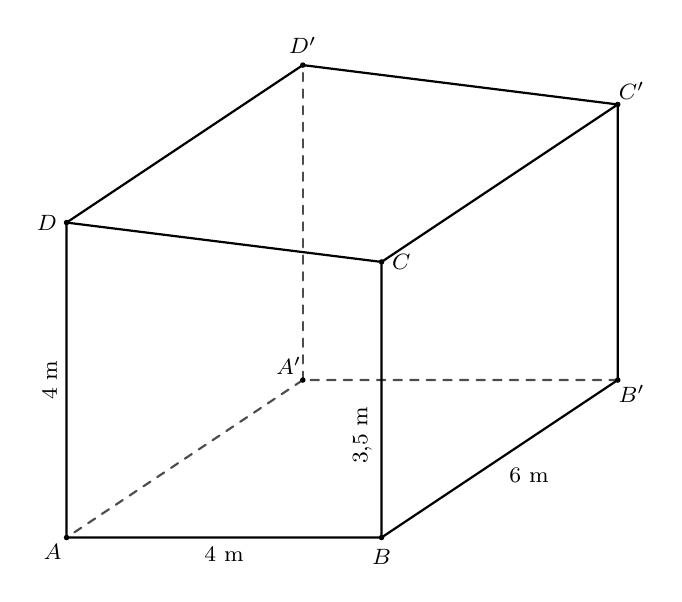
\begin{tikzpicture}[scale=1, font=\footnotesize, line join=round, line cap=round, >=stealth]
	% Định nghĩa tọa độ gốc
	\coordinate (A) at (0,0);
	\coordinate (B) at (4,0);
	\coordinate (C) at (4,3.5);
	\coordinate (D) at (0,4);
	
	% Định nghĩa vector tịnh tiến để tạo hình hộp
	\def\vx{3} 
	\def\vy{2}
	\coordinate (A') at (\vx, \vy);
	\coordinate (B') at (4+\vx, \vy);
	\coordinate (C') at (4+\vx, 3.5+\vy);
	\coordinate (D') at (\vx, 4+\vy);
	
	% Vẽ các cạnh khuất
	\draw[dashed, thick, black!70] (B') -- (A') -- (A);
	\draw[dashed, thick, black!70] (A') -- (D');
	
	% Vẽ các mặt thấy được
	\draw[thick] (A) -- (B) -- (C) -- (D) -- cycle; 
	\draw[thick] (D) -- (D') -- (C') -- (C);       
	\draw[thick] (B) -- (B') -- (C');               
	
	% Điểm và Nhãn theo quy tắc foreach chuyên gia
	\foreach \x/\g in {A/-135, B/-90, C/0, D/180, A'/135, B'/-45, C'/45, D'/90} 
	\fill[black] (\x) circle (1pt)+(\g:.25) node {$\x$};
	
	% Chú thích kích thước (Sử dụng dấu ngoặc nhọn cho số thập phân theo yêu cầu)
	\node[above, rotate=90] at (0, 2) {$4$ m};          
	\node[below] at (2, 0) {$4$ m};          
	\node[above, rotate=90] at (4, 1.3) {$3{,}5$ m};     
	\node[below right] at (5.5, 1) {$6$ m};  
\end{tikzpicture}
	}
	\par\shortans[0]{7{,}9}
	\loigiai{
	\immini{Ta trải phẳng $3$ bức tường $ADD'A'$, $ABB'A'$, $BCC'B'$ lên cùng một mặt phẳng.\\
		Chọn hệ trục tọa độ $Oxy$ sao cho $O \equiv A'$, tia $Ox$ trùng với tia $A'B'$, tia $Oy$ trùng với tia $A'A$ (hướng xuống sàn). Khi đó
		\begin{itemize}
			\item Bức tường giữa $ABB'A'$ nằm trong khoảng $x \in [0; 4]$.
			\item Bức tường trái $ADD'A'$ nằm trong khoảng $x \in [-4; 0]$.
			\item Bức tường phải $BCC'B'$ nằm trong khoảng $x \in [4; 7{,}5]$ (do rộng $3{,}5$ m).
		\end{itemize}}{
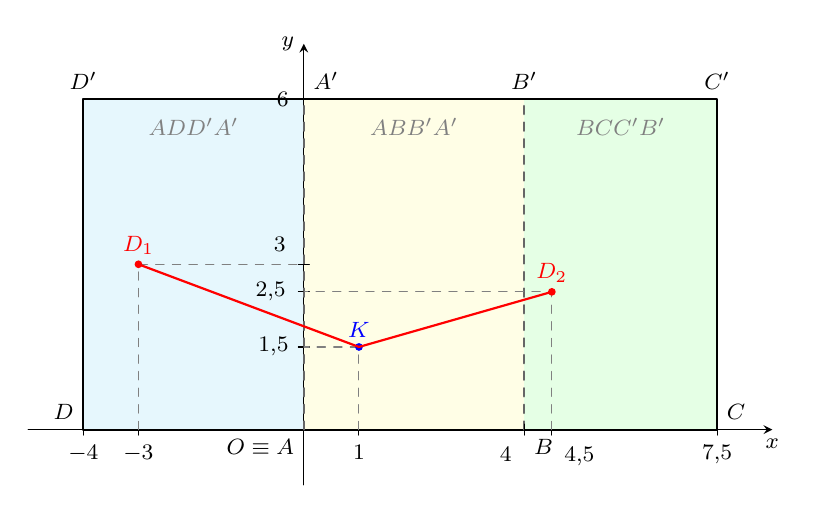
\begin{tikzpicture}[scale=0.7, font=\footnotesize, line join=round, line cap=round, >=stealth]

	\fill[cyan!10] (-4,0) rectangle (0,6);
	\fill[yellow!10] (0,0) rectangle (4,6);

	\fill[green!10] (4,0) rectangle (7.5,6);

	\draw[->] (-5, 0) -- (8.5, 0) node[below] {$x$};
	\draw[->] (0, -1) -- (0, 7) node[left] {$y$};
	
	\draw[thick] (-4,0) rectangle (7.5,6);
	\draw[dashed, thick, black!60] (0,0) -- (0,6); % Cạnh A-A'
	\draw[dashed, thick, black!60] (4,0) -- (4,6); % Cạnh B-B'
	
	\foreach \x/\t in {-4/$-4$, -3/$-3$, 1/$1$, 7.5/$7{,}5$} {
		\draw (\x, 0.1) -- (\x, -0.1) node[below] {\t};
	}
	\draw (4, 0.1) -- (4, -0.1) node[below left=1pt] {$4$};
	\draw (4.5, 0.1) -- (4.5, -0.1) node[below right=1pt] {$4{,}5$};
	
	\foreach \y/\t in {1.5/1{,}5, 6/6} {
		\draw (0.1, \y) -- (-0.1, \y) node[left] {\t};
	}
	\draw (0.1, 2.5) -- (-0.1, 2.5) node[left=1pt] {$2{,}5$};
	\draw (0.1, 3) -- (-0.1, 3) node[above left=1pt] {$3$};
	
	\draw[dashed, thin, gray] (-3,0) -- (-3,3) -- (0,3);
	\fill[red] (-3,3) circle (2pt) node[above] {$D_1$};
	
	% Điểm K (1; 1.5)
	\draw[dashed, thin, gray] (1,0) -- (1,1.5) -- (0,1.5);
	\fill[blue] (1,1.5) circle (2pt) node[above] {$K$};
	
	% Điểm D2 (4.5; 2.5)
	\draw[dashed, thin, gray] (4.5,0) -- (4.5,2.5) -- (0,2.5);
	\fill[red] (4.5,2.5) circle (2pt) node[above] {$D_2$};
	
	% --- 6. VẼ DÂY ĐIỆN (ĐƯỜNG GẤP KHÚC) ---
	\draw[thick, red] (-3,3) -- (1,1.5) -- (4.5,2.5);
	
	% --- 7. GHI CHÚ ĐỈNH VÀ TÊN TƯỜNG ---
	\node[above left] at (-4,0) {$D$};
	\node[above ] at (-4,6) {$D'$};
	\node[below left] at (0,0) {$O \equiv A$};
	\node[above right] at (0,6) {$A'$};
	\node[below right] at (4,0) {$B$};
	\node[above ] at (4,6) {$B'$};
	\node[above right] at (7.5,0) {$C$};
	\node[above] at (7.5,6) {$C'$};
	
	\node[gray] at (-2, 5.5) {$ADD'A'$};
	\node[gray] at (2, 5.5) {$ABB'A'$};
	\node[gray] at (5.75, 5.5) {$BCC'B'$};
	
\end{tikzpicture}	
	}
		Xác định tọa độ các điểm
		\begin{itemize}
			\item Bóng đèn $1$ ($D_1$). Cách sàn $3$ m nên $y = 6 - 3 = 3$. Giả sử khoảng cách ngang từ cạnh $A'D'$ (hiểu là $A'A'$) là $3$ m nên $ x = -3$. Vậy $D_1(-3; 3)$.
			\item Bảng điều khiển ($K$): Cách $A'D'$ (tức trục $Oy$) $1$ m và cách sàn $1{,}5$ m nên $x = 1$, $y = 6 - 1{,}5 = 4{,}5$ (hoặc nếu gốc $O$ ở sàn thì $y=1{,}5$).\\
			 Để khớp với hệ quy chiếu cũ (gốc tại trần $A'$ nhưng tung độ dương hướng xuống sàn hoặc ngược lại), ta dùng khoảng cách so với sàn là $y_K=1{,}5$, $y_{D1}=3$, $y_{D2}=2{,}5$.
			\item Bóng đèn $2$ ($D_2$). Cách sàn $2{,}5$ m nên $y = 2{,}5$.\\
			 Cách cạnh $B'C'$ là $3$ m, mà tường rộng $3{,}5$ m nên bóng đèn cách trục $B'B'$ ($x=4$) là $0{,}5$ m.\\
			  Vậy $x = 4 + 0{,}5 = 4{,}5$.
			  Tọa độ $D_2(4{,}5; 2{,}5)$.
		\end{itemize}
		Tổng chiều dài dây điện tối thiểu là $L = KD_1 + KD_2$ là 
		\[ L = \sqrt{(-3-1)^2 + (3-1{,}5)^2} + \sqrt{(4{,}5-1)^2 + (2{,}5-1{,}5)^2}  \approx 7{,}9. \]
	}
\end{ex}

\begin{ex}%[2D1V3-2]%[DỰ ÁN TEX ĐỀ THI THỬ THPT 2026]%[NHẬT THIỆN]
	\immini{Trong mùa mưa lũ, nước ở trên thượng nguồn đổ dồn về hạ lưu rất mạnh nên thường làm lệch quỹ đạo chuyển động của tàu, thuyền trên sông. Giả sử trong một hệ trục tọa độ $Oxy$, một chiếc thuyền đang ở tại điểm $A\left(4;\dfrac{5}{3}\right)$ chuyển động về phía gốc tọa độ $O$. Do dòng chảy mạnh nên thuyền di chuyển trên cung đường $AB$ là một phần của đồ thị hàm số $y=\dfrac{ax+b}{cx+d}$ như hình vẽ, với $B(-1;0)$. Gọi $M$ là một điểm bất kỳ nằm trên cung đường di chuyển của chiếc thuyền. Khoảng cách từ $M$ đến $O$ ngắn nhất bằng bao nhiêu? (\textit{làm tròn kết quả đến hàng phần trăm}).}
{\begin{tikzpicture}[scale=1, font=\footnotesize, line join=round, line cap=round, >=stealth]
		\def\func(#1){(2*(#1)+2)/((#1)+2)}
		\draw[->] (-1.5,0) -- (5.5,0) node[below] {$x$};
		\draw[->] (0,-0.5) -- (0,3) node[right] {$y$};
		\node[below left] at (0,0) {$O$};
		\foreach \x in {1,2,3}
		\draw (\x,0.1) -- (\x,-0.1) node[below] {\small $\x$};
		\draw (4,0.1) -- (4,-0.1) node[below] {$4$};
		\draw (0.1,1) -- (-0.1,1) node[left] {$1$};
		\draw (0.1,2) -- (-0.1,2) node[right] {$2$};
		\draw[dashed] (0, 5/3) -- (4, 5/3);
		\draw (0.1, 5/3) -- (-0.1, 5/3) node[left] {\fontsize{7pt}{0}\selectfont $\frac{5}{3}$};
		\draw[thick, teal!60!black, domain=-1:4.5, samples=100] 
		plot (\x, {\func(\x)});
		\fill[black!70] (-1,0) circle (1.5pt) node[above left] {$B$};
		\node[below] at (-1,0) {$-1$};
		\fill[black!70] (0,1) circle (1.5pt);
		\coordinate (A) at (4, {5/3});
		\draw[dashed] (4,0) -- (A);
		\fill[black!70] (A) circle (1.5pt) node[below right] {$A$};
		\begin{scope}[shift={(A)}, scale=0.4]
			\draw[fill=blue!80!black, rounded corners=1pt] 
			(-1, 0) -- (1, 0) -- (1.2, 0.4) -- (-0.8, 0.4) -- cycle;
			\draw[thick, gray] (0.2, 0.4) -- (0.2, 2.5);
			\draw[fill=white!90!gray] (0.25, 0.5) -- (1.2, 0.5) -- (0.25, 2.2) -- cycle;
			\draw[fill=gray!30] (0.15, 0.6) -- (-0.5, 0.6) -- (0.15, 1.8) -- cycle;
			\draw[fill=red] (0.2, 2.5) -- (0.6, 2.3) -- (0.2, 2.1) -- cycle;
			\node[text=white, scale=0.4] at (0.2, 0.2) {\tiny Thuyền};
		\end{scope}
\end{tikzpicture}}
	\par\shortans[0]{0{,}83}
	\loigiai{
		Hàm số $y=\dfrac{a_1x+b_1}{x+d_1}$ đi qua $A\left(4;\dfrac{5}{3}\right)$, $B(-1;0)$ và điểm cắt trục tung $(0;1)$.
		$$\heva{&\dfrac{4a_1+b_1}{4+d_1}=\dfrac{5}{3}\\ &-a_1+b_1=0 \Rightarrow a_1=b_1\\ &\dfrac{b_1}{d_1}=1 \Rightarrow b_1=d_1.}$$
		Suy ra $a_1=b_1=d_1$. Chọn $a_1=2 \Rightarrow y=\dfrac{2x+2}{x+2}$.\\
		Lấy $M\left(x;\dfrac{2x+2}{x+2}\right)$ với $-1\le x\le4$.\\
		Ta có $OM=\sqrt{x^2+\left(\dfrac{2x+2}{x+2}\right)^2}$.\\
		Xét hàm số $f(x)=x^2+\left(\dfrac{2x+2}{x+2}\right)^2$ trên đoạn $[-1;4]$.\\
		Ta có $f'(x)=2x+\dfrac{8(x+1)}{(x+2)^3}=0\Leftrightarrow x=-2+\sqrt{2}$.\\
		Xét $f(-1)=1$; $f(4)=\dfrac{169}{9}$ và $f\left(-2+\sqrt{2}\right)=12-8\sqrt{2}$.\\
		Khi đó $\min\limits_{[-1;4]} f(x)=12-8\sqrt{2}$ khi và chỉ khi $x=-2+\sqrt{2}$.\\
		Vậy ta được $\min OM\approx \sqrt{12-8\sqrt{2}}\approx 0{,}83$.
	}
\end{ex}



\Closesolutionfile{ans}
%\cautl
\Closesolutionfile{ansbook}
%\begin{indapan}
%	{ans/ans\currfilebase}
%\end{indapan}

